% !TeX root = ../report.tex
% !TeX spellcheck = en-US
% !TeX encoding = UTF-8


\section{UNDERWATER COMMUNICATION}\label{sec:underwater_communication}
This section describes various principles of underwater communication. It identifies two basic methods of
transmitting data, namely: wired communication or wireless communication. Wired communication will be in the form of
an \gls{gls-umbilical} which is an electronic cable connecting to an underwater vehicle using regular and industry
standard communication protocols. Wireless communication can be performed through four basic principles:
electromagnetic, electric current, acoustic or optical signals. Of these principles only electromagnetic and acoustic
are explored, since an electrical current doesn't work in a fresh water reservoir and optical signals get sub-optimal
performance in a dredging environment due to diffraction and scattering of light by floating sand particles.

The environment presented in the use-cases, described in Section~\ref{sec:usecases}, state that the crawler will 
operate in fresh water basins. It's also likely that it will be connected to the water surface with a floating 
\gls{gls-dredgeline}. The choice for wired communication is therefore easily made. There may, however, still be a 
need for wireless communication with external sensors (as the principles presented in 
Section~\ref{sec:coverageunderuncertainty} illustrate). Where an option to minimize a localization error using 
multiple bots, is presented.

\subsection{WIRED COMMUNICATION}\label{sec:wired communication}
With wired communication, data signals are transmitted through a wire which acts as a pathway where the information 
is transmitted as a digital \gls{gls-bitstream} (a sequential binary sequence). Transmission of information through 
this wire is limited by a certain bandwidth in \si{\hertz} were the limiting factors are material properties such as:
conductivity, permittivity and permeability. As well as processing of the signals at the end and start node, 
communication wires are made of a carrier medium, such as copper or glass fibre. This carrier medium facilitates 
transmission of electromagnetic waves or currents where electromagnetic waves, such as light, are transmitted through
fiber optic cables and a modulated pulse of light propagates through a glass tube through the principle of 
\gls{acr-TIR}. Electromagnetic communication makes use of copper wires, where an electric charge propagates through 
the cable. Copper is the industry de-facto preference due to its high-conductivity, low electrical resistance and 
resistance to corrosion.

\citet{babani_comparative_nodate} made a comparative study between fibre-optic and copper cables in a context of 
modern network protocol. They identified the following properties for comparison: bandwidth, cost, dimensional 
properties (such as weight, size and flexibility), signal loss and safety and immunity. They illustrate that fiber 
optics cables, although more expensive, are the better choice by stating that fibre-optic cables are smaller and 
lighter compared to metal cables, especially copper based. Optical fibre occupies less space in conduits than copper 
cabling, they weigh less and have a tighter bend radius than any copper cable. Furthermore, signals don't cross-talk 
with neighboring wires. The low signal attenuation performance and superior signal integrity found in fiber optical 
systems facilitates much longer runs for signal transmission. The attenuation loss experienced in fiber optic cables 
can be attributed to microscopic and macroscopic impurities in the fiber material and structure, which cause 
absorption and scattering of light signal. In figure~\ref{fig:attenuationFibreVSCopper} the attenuation loss of \( 1 
\si{\km} \) of cable is shown as a function of frequency. Both signals propagate with nearly the same speed through 
their corresponding wire, but when a high data throughput is wanted. It becomes evident from this figure that usage 
of fiber-optics are paramount.

\begin{RoyalFigure}[htb, label=fig:attenuationFibreVSCopper]{EFFECTIVE ATTENUATION FIBER VS COPPER CABLE 1 
km~\cite{joseph_c_palais_fibre_1998}}
    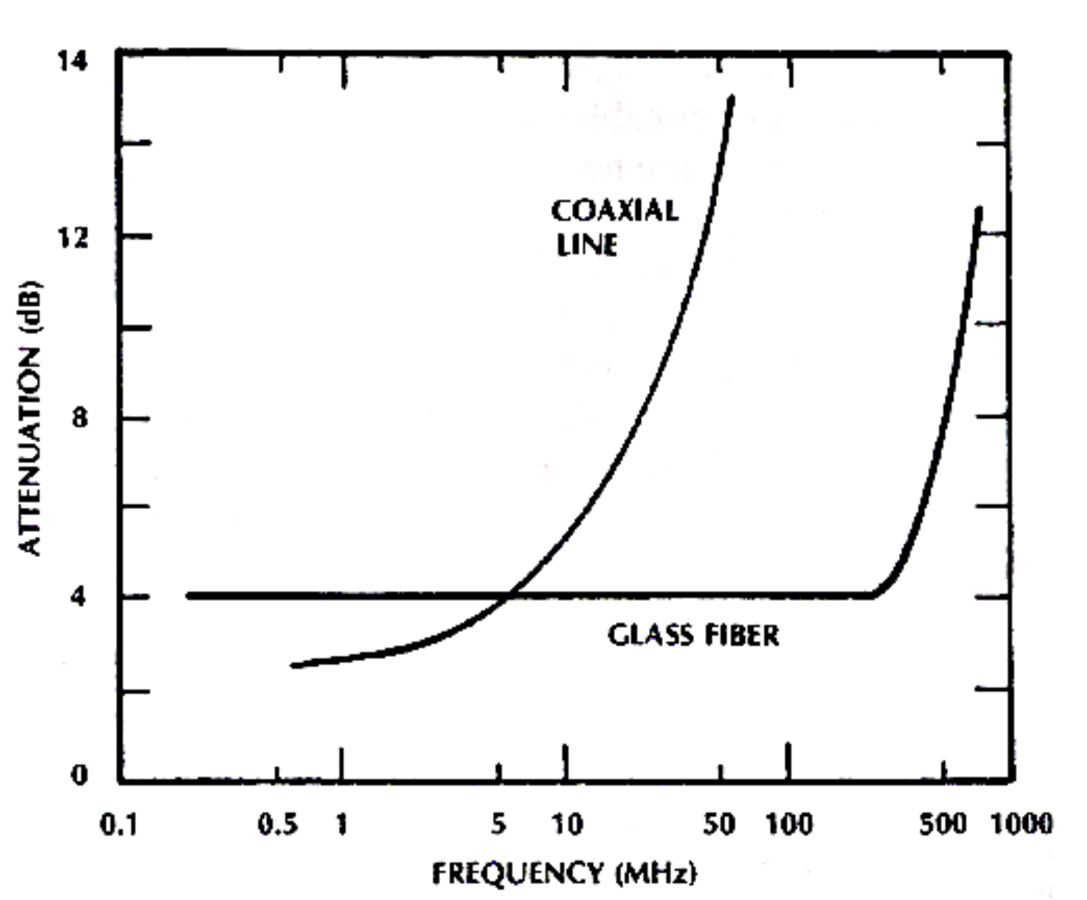
\includegraphics[width=0.75\textwidth]{attenuationFibreVSCopper.pdf}
\end{RoyalFigure}

Other important factors to consider, for an underwater wired-communication between a base station and a dredge bot, 
are the effects of the wire on the bot itself. \citet{whitcomb_underwater_2000} states that most present day vehicles
are \glspl{acr-ROV} --- tele-operated vehicles employing an \gls{gls-umbilical} cable to carry both power and 
telemetry from a mother-ship to the vehicle. He further states that a growing number of research vehicles are 
\glspl{acr-AUV} --- which operate without an \gls{gls-umbilical} tether. This statement is supported by 
\citet{valavanis_control_1997}, who describes that the \gls{acr-ROV} \gls{gls-umbilical} cable constrains the vehicle
to operations in close proximity to the support ship. Because the crawler is tethered to a location above water 
level, due to it's floating \gls{gls-dredgeline}, and because this crawler is from its starting-point constructed as 
a \gls{acr-ROV}, it will, in all likelihood, be controlled through an \gls{gls-umbilical}.

\citet{westneat_advances_1983} describes that, as the range of operations becomes longer and the water deeper, the 
drag exerted by the tether becomes significant. The thrusters, and thus the vehicle itself, must become larger and 
the cable thicker, and the energy that goes into the cable maintenance becomes a major factor. This factor is 
illustrated by \citet{fang_motions_2007}, who describes a mathematical model which allow the state representation of 
the dredge bot, as described in section~\ref{sec:state representation}, to be modified by the forces that are exerted
on the cable. In these equations, mass and inertia of the cable play an important role. Because these are just a 
fraction of the properties for a \gls{gls-dredgeline}, it's assumed that these forces can be neglected. According to 
\citet{feng_evaluation_2004}, the effects of the cable can be reduced when it's deployed by a drum on the shore with 
negligible tension when it's pulled by the vehicle.

\subsubsection*{Protocols}\label{sec:wired_protocols}
The signals which are transported through the wires need to adhere to certain rules and conventions. In other words, 
the transponder and receiver need to speak the same language and be aware of etiquette in order for a message to be 
received as intended. The \gls{acr-IEEE}, have dictated most of the widespread used norms today. The most common used
norm in wired communication is \textit{IEEE 802.3} or as it's more commonly known Ethernet. Ethernet consists of a 
multitude of protocols. In this \gls{acr-IEEE} norms are the physical layer, data link layers and the \gls{acr-MAC} 
for each protocol defined.

Shortly put, \gls{acr-MAC} is defined as the lower sub layer of the data link layer and provides addressing and 
channel access control mechanisms that allow for communication between several terminals, or nodes, within a multiple
access network. This layer acts as an interface between the \gls{acr-LLC} sub layer and the network's physical layer;
the \gls{acr-LLC} makes it possible to let several network protocols coexist. According to \citet{jolectra_plc_2016},
the current dredge bot makes use of an \textit{Allen Bradley ETHERNET/IP adapter} of type \textit{1769-AENTR}, which 
allows the use of the \gls{acr-CIP}, \gls{acr-TCP} and \gls{acr-UDP}. \gls{acr-CIP} is used by EtherNet/IP, and is a 
familiar and widely used protocol for controllers.

\subsection{WIRELESS COMMUNICATION}
\citet{freitas_evaluation_2014} tells us that wireless communications have been subject to enormous research and 
improvements in the near past. This effort is responsible for allowing multiple devices to securely communicate 
simultaneously with high availability, great distances and high data rates. While these improvements are applied and 
tested mainly in over-the-air communications, underwater communications suffer from a low applicability of radio 
frequency transmission systems due to a low attenuation of \gls{acr-EMW}  in water.

He~\cite{freitas_evaluation_2014} further states that when using radio frequency, underwater communications do not 
fully benefit from the improvements achieved in air due to the fact that electromagnetic propagation in water causes 
a vast reduction in the range of communcation. Because of the limitations that water imposes, these communications 
are currently performed using acoustic waves and in some cases optical systems. This is further supported by 
\citet{lloret_underwater_2012} who remarks that underwater communication research is primarily focused on the use of 
optical signals, electromagnetic signals and the propagation of acoustic and ultrasonic signals. Each technique has 
its own characteristics, with its benefits and drawbacks, mainly due to the chemical 
characteristics~\cite{garcia_underwater_2011} and physical constraints of the medium~\cite{lanbo_prospects_2008}.

\subsubsection{ELECTROMAGNETIC COMMUNICATION}\label{sec:em}
A common method to transfer data via a wireless connection is to make use of \gls{acr-EMW}, this is a type of 
electromagnetic radiation with wavelengths in the electromagnetic spectrum (as is shown in 
figure~\ref{fig:emspectrum}). Waves in this spectrum can have frequencies between \( 3 \si{\kilo\hertz} \) or \( 3 
\si{\giga\hertz} \). These waves travel the speed of light and are transverse waves, because the amplitude is 
perpendicular to the direction of the wave travel. However, \gls{acr-EMW} are always waves of fields, not of matter, 
because they are fields, \gls{acr-EMW} can propagate in empty space~\cite{giancoli_physics_2015}.

\begin{RoyalFigure}[!htb, label=fig:emspectrum]{ELECTROMAGNETIC SPECTRUM~\cite{giancoli_physics_2015}}
    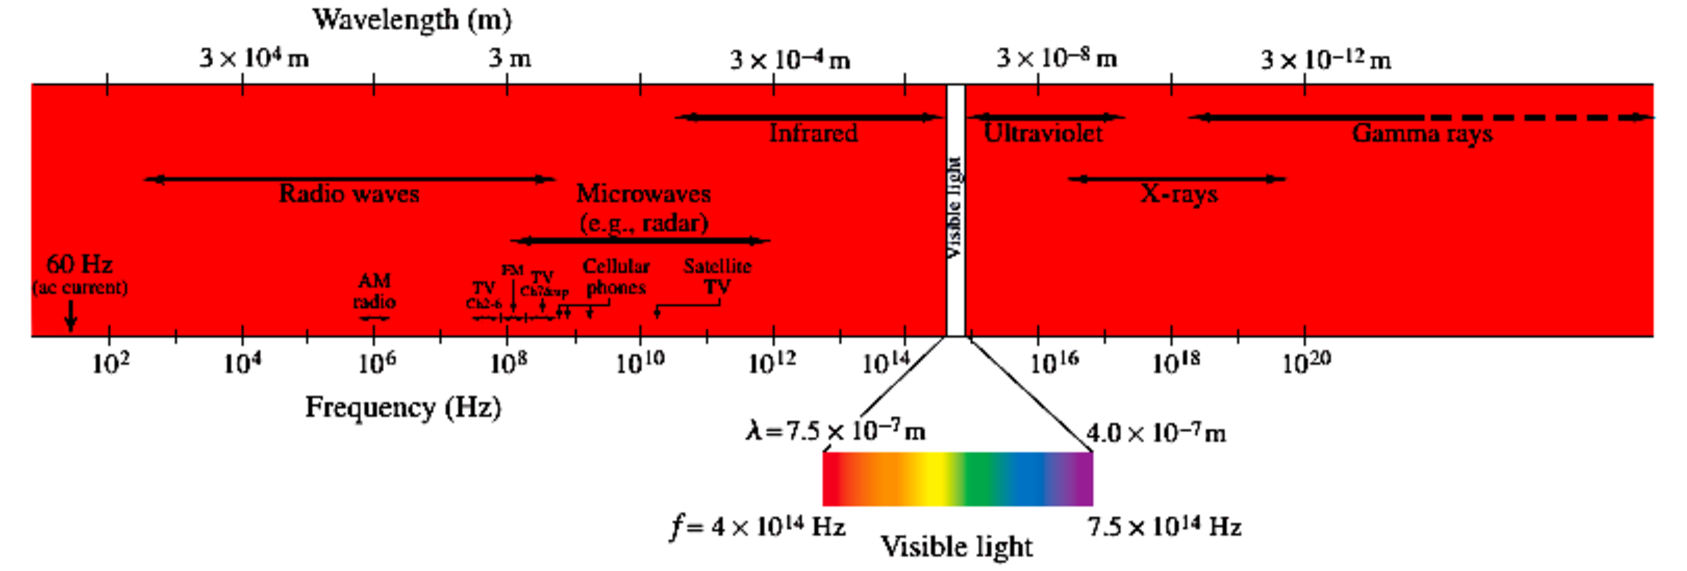
\includegraphics[width=\textwidth]{emspectrum.pdf}
\end{RoyalFigure}

Data is transferred between devices by either modulating the frequency or altering the amplitude of a signal to carry
the data. Where a carrier frequency is modulated by superimposing a data signal. This is illustrated in 
figure~\ref{fig:AMFM}.

\begin{RoyalFigure}[htb, label=fig:AMFM]{SIGNAL MODULATION}
    \begin{tcbraster}[raster columns=2, raster equal height]
        \begin{tikzpicture}
            \begin{axis}[%
            title=\usekomafont{captionlabel}\color{RoyalBlack}AMPLITUDE MODULATION (AM),%
            domain=0:10,%
            samples=500,%
            legend entries={carrier, data, signal}%
            ];%
                \addplot[thin, RoyalBlack]{cos(deg(pi*x/3))};%
                \addplot[thin, RoyalBlack]{cos(deg(pi*x*4))/2};%
                \addplot[thick, RoyalRed]{cos(deg(pi*x/3))+cos(deg(pi*x*4))/2};%
            \end{axis}
        \end{tikzpicture}
        \begin{tikzpicture}
            \begin{axis}[%
            title=\usekomafont{captionlabel}\color{RoyalBlack}FREQUENCY MODULATION (FM),%
            domain=0:10,%
            samples=500,%
            legend entries={carrier, data, signal}];%
                \addplot[thin, RoyalBlack]{cos(deg(pi*x/3))};%
                \addplot[thin, RoyalBlack]{cos(deg(pi*x*4))/2};%
                \addplot[thick, RoyalRed]{cos(deg(pi*cos(deg(pi*x/3))*4))/2};%
            \end{axis}
        \end{tikzpicture}
    \end{tcbraster}
\end{RoyalFigure}

\citet{hagman_elias_design_2009} tells us that the reasons why \gls{acr-EMW} are used to transfer information in the 
classic wireless air channel lies in their fast propagation speed, their wide usable frequency spectrum and the small
amount of environment noise created compared, for example with acoustics factors. This all leads to the possibility 
of high data rates. Furthermore, the \gls{acr-EMW} has the ability to propagate without a carrier medium and the 
electric-magnetic field conversion enables in general very large communication ranges.

But in water --- especially in seawater --- things are much different. This statement is supported by 
\citet{ramakrishna_next_2012} when they convey that the ocean is almost impervious to \gls{acr-EMW}, which makes them
useless for wireless underwater communication over distances greater than a hundred meters. 
\citet{hagman_elias_design_2009} illustrated this by solving \gls{gls-maxwell} to predict the propagation of 
\gls{acr-EMW} for the case of a linearly \gls{gls-polarized-plane} travelling in \(z\)-direction, we get the 
\gls{gls-electric-field} strength \gls{sym-E_x}  and the \gls{gls-magnetic-field} strength 
\gls{sym-H_y}~\cite{hagman_elias_design_2009}.

\begin{RoyalFigure}[!htb, label=fig:elecmagdamp]{DAMPENING OF ELECTRIC AND MAGNETIC FIELD}
    \begin{tikzpicture}[x={(-10:1cm)},y={(90:1cm)},z={(210:1cm)},scale=2.0]
        % Axes
        \draw[->] (-1,0,0) node[above] {$z$} -- (5,0,0);
        \draw[->] (0,0,0) -- (0,2,0) node[above] {$x$};
        \draw[->] (0,0,0) -- (0,0,2) node[left] {$y$};
        % Propagation
        \draw[->, thick] (5,0,0) -- node[above] {\gls{sym-gamma_EM} } (6,0,0);
        % Waves
        \draw[RoyalRed,thick] plot[domain=0:4.5,samples=200] (\x,{2*cos(deg(pi*\x))/(\x/2+1)},0);
        \draw[RoyalRed,thick] plot[domain=0:4.5,samples=200] (\x,0,{2*cos(deg(pi*\x))/(\x/2+1)});
        % Arrows
        \foreach \x in {0.1,0.3,...,4.4} {
        \draw[->,help lines,RoyalRed] (\x,0,0) -- (\x,{2*cos(deg(pi*\x))/(\x/2+1)},0);
        \draw[->,help lines,RoyalRed] (\x,0,0) -- (\x,0,{2*cos(deg(pi*\x))/(\x/2+1)});
        }
        % Labels
        \node[above right] at (0.5,1.8,0) {\( \gls{sym-E_hat} \)};
        \node[below] at (0.5,0,1.8) {\( \gls{sym-H_hat} \)};
    \end{tikzpicture}
\end{RoyalFigure}

\gls{sym-E_hat}  and \gls{sym-H_hat} are the amplitudes of the electric and the magnetic field wave and 
\gls{sym-gamma_EM} is the propgation constant, expressed in \gls{sym-epsilon_e}, which is the permittivity, as shown 
in equation~\ref{eq:propegationconst}, \gls{sym-mu_e} is the electromagnetism permeability and \gls{sym-sigma_e} is 
the electrical conductivity of a material. Here \gls{sym-alpha_e} is the attenuation and \gls{sym-beta} the phase 
factor of a wave.

\begin{equation}
    \label{eq:MaxwellE}
    \gls{sym-E_x} = \gls{sym-E_hat} \gls{sym-exp}^{\gls{sym-imag}  \gls{sym-omega}  \gls{sym-t}  - \gls{sym-gamma_EM}
    z}
\end{equation}

\begin{equation}
    \label{eq:MaxwellH}
    \gls{sym-H_y}  = \gls{sym-H_hat} \gls{sym-exp}^{\gls{sym-imag}  \gls{sym-omega}  \gls{sym-t}  - 
    \gls{sym-gamma_EM}  z}
\end{equation}

\begin{equation}
    \label{eq:propegationconst}
    \gls{sym-gamma_EM}  = \gls{sym-imag}  \gls{sym-omega}  \sqrt{\gls{sym-epsilon_e}  \gls{sym-mu_e}  - 
    \frac{\gls{sym-imag}
    \gls{sym-sigma_e}  \gls{sym-mu_e} }{\gls{sym-omega} }} = \alpha + \gls{sym-imag} \gls{sym-beta}
\end{equation}

\begin{equation}
    \label{eq:attfactor}
    \gls{sym-alpha_e}  \approx 0.0173 \sqrt{f \gls{sym-sigma_e} }
\end{equation}

As is evident from equation~\ref{eq:MaxwellE} and~\ref{eq:MaxwellH}, there is a logarithmic relationship; 
maximization of the propagation \gls{sym-gamma_EM} leads to a lower amplitude of the electric and magnetic fields. 
This propagation is mostly determined by the attenuation \gls{sym-alpha_e}, which varies at different frequencies and
mediums. \citet{claus_design_2014} tells us that this attenuation factor is given as equation~\ref{eq:attfactor}, 
which shows us that the attenuation is related to the square root of the frequency \( f \) multiplied by the 
conductivity of the water \gls{sym-sigma_e}. \citet{hattab_underwater_2013} states that the loss of a signal 
travelling through water can be calculated using equation~\ref{eq:attloss}. They state that the knowing the real-part
of \gls{sym-gamma_EM} is sufficient to calculate the loss for a given frequency. Since the only changing term, due to
frequency in the complex-valued \gls{sym-gamma_EM}, is in its imaginary part, and due to the fact that each 
\gls{sym-gamma_EM} is multiplied with \gls{sym-imag}, both outside of the root as inside, this value will be a 
constant throughout the frequency spectrum. This attenuation model will not be used for our calculations where 
\gls{sym-Delta_d_1_2} is the separation distance between transmitting and receiving nodes and only the real part of 
the propagation constant \gls{sym-sigma_e} is used.

\begin{equation}
    \label{eq:attloss}
    \gls{sym-L_alpha_epsilon} = \Re(\gls{sym-gamma_EM}) = \frac{20}{\ln(10)} \gls{sym-Delta_d_1_2} \Rightarrow
    \gls{sym-Delta_d_1_2} \frac{\gls{sym-L_alpha_epsilon}}{\Re( \gls{sym-gamma_EM} )\frac{20}{\ln(10)}} = 
    \frac{\gls{sym-L_alpha_epsilon} }{\gls{sym-alpha_e} }
\end{equation}

The maximum penetration depth of signal in (sea) water, will, for simplicity’s sake be calculated with 
equation~\ref{eq:attloss}, where \gls{sym-alpha_e} is obtained using equation~\ref{eq:attfactor}.
\citet{jiang_electromagnetic_2011} tells us that seawater has a typically high conductivity of 
\SI{4}{\siemens\per\meter}, whilst freshwater has a typically conductivity of only \SI{0.01}{\siemens\per\meter}, 
\num{400} times less.
He~\cite{jiang_electromagnetic_2011} further states that communication using electromagnetic waves in fresh water can
be more efficient in fresh water.
This statements are confirmed by \citet{jiang_electromagnetic_2011},~\citet{ainslie_principles_2010} 
and~\citet{bogie_conduction_1972}.
Figure~\ref{fig:propagationrange} and~\ref{fig:propagationrange_wifi}, which shows the \gls{acr-EMW} propagation in 
fresh and seawater for commonly used frequencies, illustrate this phenomenon.

\subsubsection{PROTOCOLS}
Subsection~\ref{sec:wired_protocols} describes the need for a transceiver and receiver to speak the same language and
adhere to the same etiquette. This holds true for wireless protocols as well. Most wireless protocols are described 
in the \gls{acr-IEEE} 802 standards. These are a family of standard network protocols describing networks carrying 
variable-size packets. These protocols are the de-facto industry standards. A short description for the most popular 
802 standards are given below. These protocols map two layers, namely: a data link layer and physical layer. The data
link layer is split into two sublayers: \gls{acr-LLC} and \gls{acr-MAC}. \gls{acr-LLC} provides the multiplexing 
mechanisms that enable the network protocols and provide flow control and automatic repeat requests whilst 
\gls{acr-MAC} provides addressing and channel access control mechanisms that makes it possible for several nodes to 
communicate within a multiple access network.

\paragraph{IEEE 802.11 WLAN} \hfil \\
The IEEE 802.11 standard is also known as WiFi. It encompasses wireless modulation techniques, designated as 802.11 
(a, b, g, n and ac). The 802.11 standard makes use of the \SI{2.4}{\giga\hertz} and \SI{5}{\giga\hertz} 
\gls{gls-bandwidth}. \citet{freitas_evaluation_2014} states that Wi-Fi frequencies maybe a challenge when used in 
underwater communications, because its attenuation drastically reduces the channel distance, as is shown in 
figure~\ref{fig:propagationrange_wifi}. A new standard 802.11af is being developed. This standard will make use of 
the \SI{700}{\mega\hertz} $ 700 [MHz] $ frequency which might give an extra couple of meters underwater.

\begin{RoyalFigure}[!htb, label=fig:propagationrange_wifi]{PROPAGATION RANGE OF WI-FI IN WATER.}
    \begin{tikzpicture}
        \begin{axis}[%
        xlabel={Frequency \si{\hertz}},%
        ylabel={Range \si{\meter}},%
        xmin=10e7,%
        xmax=10e9,%
        xmode=log,%
        grid=major,%
        xminorgrids=true,%
        width=\textwidth,%
        height=0.5\textwidth,%
        extra x ticks={700e6,2.4e9,5e9},%
        extra x tick labels={\SI{700}{\mega\hertz}, \SI{2.4}{\giga\hertz}, \SI{5}{\giga\hertz}},%
        extra x tick style={%
        xticklabel style={yshift=-0.5ex,xshift=-1cm, anchor=south}%
        }];%
            \addplot[mark=none, color=RoyalRed, thick, dashed] file {resources/range_sea_802_11.dat};%
            \addlegendentry{Sea water \(\gls{sym-sigma_e} = \SI{4}{\siemens\per\meter} \)};%
            \addplot[mark=none, color=RoyalRed, thick] file {resources/range_fresh_802_11.dat};%
            \addlegendentry{Fresh water \(\gls{sym-sigma_e} = \SI{1e-2}{\siemens\per\meter} \)};%
            \draw (axis cs:700e6,-10) -- (axis cs:700e6,15);%
            \draw (axis cs:2.4e9,-10) -- (axis cs:2.4e9,15);%
            \draw (axis cs:5e9,-10) -- (axis cs:5e9,15);%
        \end{axis}
    \end{tikzpicture}
\end{RoyalFigure}

\paragraph{IEEE 802.15.4 LO-FI} \hfill \\
From all different protocols described in the \gls{acr-IEEE} 802.15 special consideration is made into the 
\gls{acr-IEEE} 802.15.14 or \gls{gls-lora} which is an upcoming communication protocol for \gls{acr-IoT} devices. It 
operates in \SI{433}{\mega\hertz} and \SIrange{863}{870}{\mega\hertz}. The protocols are opensource and the modules 
are very cheap. This protocol is developed for robust, long range communication which can reach \SI{22}{\kilo\meter} 
on land. \citet{akyildiz_underwater_2005} tell us that the electromagnetic waves at \SI{433}{\mega\hertz} have been 
reported to have a transmission range of \SI{120}{\cm} in an underwater environment. These experiments have been 
performed at the \gls{acr-RESL} at the University of Southern California.

Because of the use of lower frequencies, \gls{gls-lora} shows a three-fold increase in range compared with normal 
WiFi. The propagation of \gls{gls-lora} signal in (sea)water is shown in figure~\ref{fig:propagationrange}.
When this is compared with figure~\ref{fig:propagationrange_wifi}, an increase in range is found.

\begin{RoyalFigure}[!htb, label=fig:propagationrange]{PROPAGATION RANGE OF LO-FI IN WATER}
    \begin{tikzpicture}
        \begin{axis}[%
        title=Propagation range of electromagnetic waves in water,%
        xlabel={Frequency \si{\hertz}},%
        ylabel={Range \si{\meter}},%
        xmin=10e6,%
        xmax=10e8,%
        xmode=log,%
        grid=major,%
        xminorgrids=true,%
        width=\textwidth,%
        height=0.5\textwidth,%
        extra x ticks={168e6,433e6,863e6},%
        extra x tick labels={\SI{168}{\mega\hertz}, \SI{433}{\mega\hertz}, \SI{863}{\mega\hertz}},%
        extra x tick style={%
        xticklabel style={yshift=-0.5ex,xshift=-1cm, anchor=south}%
        }];%
            \addplot[mark=none, color=RoyalRed, dashed, thick] file {resources/range_sea_EM.dat};%
            \addlegendentry{Sea water \(\gls{sym-sigma_e} = \SI{4}{\siemens\per\meter} \)};%
            \addplot[mark=none, color=red, thick] file {resources/range_fresh_EM.dat};%
            \addlegendentry{Fresh water \(\gls{sym-sigma_e} = \SI{1e-2}{\siemens\per\meter} \)};%
            \draw (axis cs:168e6,-100) -- (axis cs:168e6,320);%
            \draw (axis cs:433e6,-100) -- (axis cs:433e6,320);%
            \draw (axis cs:863e6,-100) -- (axis cs:863e6,320);%
        \end{axis}
    \end{tikzpicture}
\end{RoyalFigure}

\subsubsection{ELECTRIC CURRENT}\label{sec:ec}
Another way to communicate is through the use of electric current. \citet{hagman_elias_design_2009} describes that 
seawater, as a conductive medium, can be subject to a modulated signal generated by a pair of transmitting electrodes
that launch a current field in the channel. If this current field is strong enough, the receiver --- that also uses a
pair of electrodes --- could measure a potential difference and therefore receive the signal. Since electric current 
noise is extremely low in seawater, small current field amplitudes are sufficient to receive information and a large 
data rate is achievable~\cite{hagman_elias_design_2009}. Since this type of transmission only works in a conductive 
medium, and the use case only specifies that a dredge bot will be deployed in fresh water basins, electric current 
communication is not deemed a viable candidate.

\subsubsection{ACOUSTIC COMMUNICATION}\label{sec:ac}

As is shown in Section~\ref{sec:em}, \gls{acr-EMW} have a very limited range in (sea) water, due to a high 
attenuation. Multiple sources such as \citet{hagman_elias_design_2009}, \citet{claus_design_2014} and 
\citet{domingo_overview_2012} state that acoustic communication is therefore the preferred way. This type of 
communication makes use of \gls{acr-SW}, or \gls{acr-AW}, which are often described as the vibration of molecules of 
the medium in which it travels --- that is, in terms of the motion or displacement of the molecules. \gls{acr-SW}  
can also be analysed from the point of view of pressure. Indeed, longitudinal waves are often called pressure waves. 
The pressure variation is usually easier to measure than the displacement~\cite{giancoli_physics_2015}. This 
principle is used by hydrophones; these are, in effect, microphones designed to be used underwater using 
piezoelectric transducers to convert pressure waves into electricity. Although acoustic communication is the 
preferred method, there are a lot of challenges to overcome. According to~\citet{tetley_electronic_2007} transmitting
and receiving acoustic energy in seawater is affected by the often unpredictable ocean environment. 
\citet{lanbo_prospects_2008} and~\citet{edward_tucholski_underwater_2006} both state that the speed of sound in the 
sea is not constant, but a function of temperature, pressure and salinity \( v(T, P, S) \). Because the speed is not 
constant sound does not travel in a straight line. Acoustic communication can can be summarized as follows:

\begin{RoyalTable}{X[2,l,m] X[4,l,m]}
    \RoyalHeader{PARAMETER|VALUE}
    \RoyalRow{Attenuation|A variable factor related to the transmitted power, the frequency of transmission, salinity of
    the seawater and the reflective consistency of the ocean floor.}
    \RoyalRow{Salinity of seawater|A variable factor affecting both the velocity of the \gls{acr-AW} and its
    attenuation.}
    \RoyalRow{Velocity of sound in salt water|This is another variable parameter. Acoustic wave velocity is precisely
    \SI{1505}{\meter\per\second} at \SI{15}{\degreeCelsius} and atmospheric pressure, but most echo-sounding equipment
    is calibrated at \SI{1500}{\meter\per\second}}
    \RoyalRow{Reflective surface of the seabed|The amplitude of the reflected energy varies with the consistency of the
    ocean floor.}
    \RoyalRow{Noise|Either inherent noise or that produced by one’s own transmission causes the signal-to-noise ratio to
    degrade, and thus weak echo signals may be lost in noise.}
    \RoyalRow{Frequency of transmission|This will vary with the system, i.e. depth sounding or Doppler speed log.}
    \RoyalRow{Angle of incidence of the propagated beam|The closer the angle to vertical the greater will be the energy reflected by the seabed.}
\end{RoyalTable}
\clearpage